\documentclass{article}

% NeurIPS 2026 style. [preprint] prints "Preprint" in the footer instead of the
% anonymous submission notice; use [final] for a camera-ready look.
\PassOptionsToPackage{numbers,sort&compress}{natbib}
\usepackage[preprint]{neurips_2026}

\usepackage[utf8]{inputenc}
\usepackage[T1]{fontenc}
\usepackage{hyperref}
\usepackage{url}
\usepackage{booktabs}
\usepackage{amsfonts,amsmath}
\usepackage{nicefrac}
\usepackage{microtype}
\usepackage{xcolor}
\usepackage{graphicx}
\usepackage{subcaption}
\usepackage{enumitem}
\usepackage{tikz}
\usetikzlibrary{positioning,arrows.meta,shapes.geometric}

\graphicspath{{figures/}}
\hypersetup{colorlinks=true,linkcolor=blue!50!black,citecolor=blue!50!black,urlcolor=blue!50!black}
\setlist{itemsep=1pt,topsep=3pt}
\newcommand{\R}[1]{\textsf{R#1}}

\title{Can Physics or Statistics Fix How AI Weather Models\\Underestimate Record-Breaking Extremes?\\
A Case Study of GraphCast on the Records of 2020}

\author{%
  Roman Gorelskii\\
  Mohamed bin Zayed University of Artificial Intelligence (MBZUAI)\\
  Abu Dhabi, United Arab Emirates
}

\begin{document}

\maketitle

\begin{abstract}
Machine-learning weather models now match traditional physics-based forecasts on everyday
weather, but they forecast record-breaking heat, cold and wind as too mild, and the more a record is broken, the worse they do.
We test two remedies proposed in the recent literature on GraphCast\_small, a
1$^\circ$ version of DeepMind's GraphCast: (i) a statistical post-processing step inspired by the
probabilistic bias correction (PBC) of Guan et al., and (ii) the global mass, moisture and energy
conservation schemes of Sha et al., built into the model and fine-tuned on an H100 cluster.
To obtain a clean test set we first detect every record of 2020 in the ERA5 reanalysis and
use three unsupervised methods to turn them into events: DBSCAN groups record cells into
space--time events, an Isolation Forest flags the record-shattering ones, and K-means on
500\,hPa height patterns assigns each event a weather regime. On 14 case-study events
(10{,}766 record cell-times) neither remedy reduces the underestimation. The statistical correction improves ordinary
forecasts but pulls uncertain forecasts toward normal conditions, which makes heat records 7 days ahead 2.3\,K worse.
Mass and moisture conservation close their budgets exactly, remove a slow moistening drift of the
model and cost no skill on 52 ordinary dates, yet leave records unchanged. Energy conservation, which relies on
learned fluxes, degrades both records and ordinary forecasts. The only gain, about 1\,K for heat
records 7 days ahead, comes from fine-tuning that made forecasts less smooth. Our results suggest that
underestimated extremes are a problem of smoothing and of the tails of the distribution, not of global physical balance.
\end{abstract}

% =====================================================================
\section{Overview}
\label{sec:overview}

\paragraph{Weather forecasting in one paragraph.}
A weather forecast starts from the best estimate of the atmosphere \emph{now} (temperature, wind,
humidity and pressure on a grid covering the globe and several heights) and steps it forward in
time. Traditional \emph{numerical weather prediction} (NWP) does this by solving the equations of
fluid dynamics and thermodynamics on supercomputers~\cite{bauer2015quiet}. Since 2023, \emph{AI weather models}
such as GraphCast~\cite{lam2023graphcast}, Pangu-Weather~\cite{bi2023pangu} and FuXi~\cite{chen2023fuxi}
learn the same step directly from 40 years of past weather. They run on one GPU in about a minute, against hours
on a supercomputer, and they score as well as or better than NWP on standard error metrics~\cite{rasp2024wb2,benbouallegue2024rise}.

\paragraph{The problem: extremes that have never happened before.}
Weather forecasts matter most on the days when something unprecedented happens: a heatwave hotter than any on
record, a cold snap, a windstorm. Zhang et al.~\cite{zhang2026records} recently showed that AI models
systematically forecast such \emph{record-breaking} events as too mild, and that physics-based models do
better here. The error grows with how far the old record is beaten, so the most unprecedented
(\emph{record-shattering}~\cite{fischer2021shattering}) events are forecast worst.
There are two intuitive reasons. First, a record lies by definition outside the range of the training data,
which a learned model cannot easily extrapolate beyond. Second, models trained to minimise squared error learn
to \emph{hedge}: when the future is uncertain, the forecast with the lowest average squared error is a smooth
average of the possible outcomes, and averages are never extreme.

\paragraph{Two candidate remedies.}
The literature offers two very different fixes, and this project asks whether either of them helps at the extremes.
\begin{enumerate}[leftmargin=*]
  \item \textbf{Statistics after the fact.} Guan et al.~\cite{guan2026pbc} correct AI and NWP forecasts with a
  \emph{probabilistic bias correction} (PBC) learned from the model's past errors, and report large gains.
  If the model is consistently too mild, learning that error and adding it back might reduce the shortfall.
  \item \textbf{Physics inside the model.} Sha et al.~\cite{sha2025conservation} make an AI model obey global
  conservation of dry-air mass, water and total energy, the same laws that NWP models solve.
  If extremes are missed because the AI model produces physically inconsistent states, enforcing the
  physics might help.
\end{enumerate}

\paragraph{What we did.}
We built an end-to-end, reproducible pipeline (Figure~\ref{fig:pipeline}) around GraphCast\_small: find every
record of 2020 in reanalysis data, group the records into events with unsupervised learning, forecast the
events with the original model (\R{0}), with three statistical corrections, and with four fine-tuned
physics-constrained versions (\R{1}--\R{4}), and compare them on the same records. We also check that the
remedies do no harm on 52 ordinary dates of 2020.

\paragraph{Contributions.}
\begin{itemize}[leftmargin=*]
  \item An event catalogue of the 2020 records built with DBSCAN, Isolation Forest and K-means (1{,}220 events, 91 record-shattering; Section~\ref{sec:events}).
  \item A controlled test of a PBC-inspired correction, with event-level bootstrap and probabilistic checks (Section~\ref{sec:res-pbc}).
  \item To our knowledge, the first implementation of Sha et al.'s conservation schemes inside GraphCast, with a control run that separates physics from fine-tuning (Sections~\ref{sec:physics}, \ref{sec:res-physics}).
  \item Evidence that neither remedy helps records, and that \emph{smoothing} is the main lever (Section~\ref{sec:conclusions}).
\end{itemize}

\begin{figure}[t]
\centering
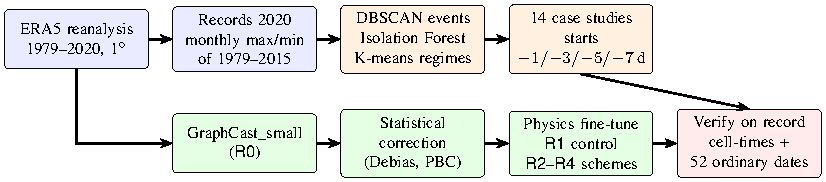
\includegraphics[width=0.92\linewidth]{pipeline.pdf}
\caption{The project pipeline. Blue: data. Orange: finding extreme events with the three unsupervised methods.
Green: forecasting systems compared. Red: evaluation on the same record cell-times, plus a ``do no harm'' check on ordinary weather.}
\label{fig:pipeline}
\end{figure}

% =====================================================================
\section{Literature review}
\label{sec:lit}

\paragraph{AI weather prediction.}
GraphCast~\cite{lam2023graphcast} is a graph neural network that maps the state of the atmosphere at two
consecutive times (6\,h apart) to the state 6\,h later. Applied repeatedly to its own output (``rolled out''),
it produces a 10-day forecast in 40 steps. Trained on ERA5 with a squared-error loss, first on single steps and then on rollouts of up to 12 steps,
it outperformed the ECMWF high-resolution forecast on 90\% of 1{,}380 verification targets. Pangu-Weather~\cite{bi2023pangu} and FuXi~\cite{chen2023fuxi} use
transformers and reach similar skill; WeatherBench~2~\cite{rasp2024wb2} provides the common data and scores. A known side effect
of squared-error training is \emph{blurring}: as uncertainty grows with lead time, forecasts become smoother than
reality. Generative models such as GenCast~\cite{price2025gencast} avoid this by producing ensembles of sharp samples.

\paragraph{AI models and extremes.}
Early evaluations found AI models competitive for many extremes, but with damped peak intensities
(e.g.\ Olivetti and Messori~\cite{olivetti2024extremes} for GraphCast and Pangu-Weather against ECMWF's IFS).
Zhang et al.~\cite{zhang2026records} focused on \emph{record-breaking} events of 2018--2023 and found that all AI models
tested underestimate both their frequency and their intensity, more so for larger exceedances, whereas the physics-based
HRES does not show this growth. Fischer et al.~\cite{fischer2021shattering} showed that record-shattering
events become more likely in a warming climate, which makes this weakness practically important.

\paragraph{Statistical post-processing.}
Correcting a model's systematic errors with statistics learned from past forecasts (``hindcasts'') is standard
practice~\cite{wilks2011statistical}. Guan et al.~\cite{guan2026pbc} propose \emph{probabilistic bias correction}
for subseasonal forecasts (weeks 3--4). It combines a debiased forecast with a persistence-based
regression on the observed starting state and outputs probabilities of five quintile categories, learned from about 20 years of reforecasts.
It strongly improves skill for both AI and dynamical models.

\paragraph{Physical constraints in neural networks.}
Constraints can be imposed through the loss (``soft'') or through the architecture (``hard''); Beucler et al.~\cite{beucler2021enforcing}
showed that hard constraints can enforce conservation exactly without loss of skill. Sha et al.~\cite{sha2025conservation}
apply hard, post-hoc fixers to an AI weather model: after every step, small multiplicative corrections restore global
dry-air mass, the global water budget (precipitation versus evaporation) and the total energy budget (top-of-atmosphere and
surface fluxes). They report more physically consistent long rollouts at no cost in skill.

\paragraph{Unsupervised learning for extremes.}
DBSCAN~\cite{ester1996dbscan} finds clusters of arbitrary shape as regions of high point density and labels isolated
points as noise, which suits events whose number and shape are unknown in advance. Isolation Forest~\cite{liu2008isolation}
detects anomalies by how quickly random splits isolate a point. K-means~\cite{lloyd1982kmeans} on principal components
of 500\,hPa height is a classical way to define \emph{weather regimes}~\cite{michelangeli1995regimes}, recurring large-scale
circulation patterns such as blocking highs. The silhouette score~\cite{rousseeuw1987silhouettes} helps choose the number of clusters.

\paragraph{Gap addressed here.}
Neither PBC nor conservation schemes have been evaluated on record-breaking extremes, and the conservation schemes have
not been implemented in GraphCast. This study runs both on the same records, with a control that separates the effect
of the physics from the effect of fine-tuning.

% =====================================================================
\section{Data}
\label{sec:data}

\paragraph{ERA5: the ``truth''.}
ERA5~\cite{hersbach2020era5} is a \emph{reanalysis}: ECMWF's best reconstruction of the global atmosphere every hour since 1940,
made by combining past observations with a physics model. We use the WeatherBench~2 copy~\cite{rasp2024wb2} (0.25$^\circ$, 6-hourly)
and take every 4th grid point, giving exactly the 1$^\circ$ grid ($181\times360$ points) that GraphCast\_small was trained on. Phase~0
verified that this reproduces the authors' example forecast exactly (2\,m temperature RMSE 1.04\,K against 3.69\,K for persistence),
with identical numbers on a laptop, Google Colab and the cluster.

\paragraph{The model.}
GraphCast\_small~\cite{lam2023graphcast} is the public 1$^\circ$ version of GraphCast with 13 pressure levels (50--1000\,hPa), trained on ERA5 1979--2015.
It predicts 6 surface variables (2\,m temperature, 10\,m wind components, sea-level pressure, 6\,h precipitation)
and 6 variables on each level (temperature, wind, geopotential, humidity). We use the authors' code (JAX, bfloat16).
Because 2020 lies outside its training years, it is a fair test year.

\paragraph{Energy and water fluxes.}
The conservation schemes need fluxes that GraphCast does not predict: evaporation, net solar and thermal radiation at the top of the atmosphere and at the surface,
and sensible and latent heat flux. We took them from ARCO-ERA5 (hourly, summed to 6\,h) for 2010--2015, about 130\,GB at 1$^\circ$.
33 isolated missing cells were filled from their neighbours.

\paragraph{Variables studied.}
Heat and cold extremes use 2\,m temperature; wind extremes use 10\,m wind speed $\sqrt{u^2+v^2}$. Records are computed over land between 60$^\circ$S and 90$^\circ$N.

% =====================================================================
\section{Methodology}
\label{sec:method}

\subsection{From records to events: the extreme-value identification}
\label{sec:events}

\paragraph{Step 1: what counts as a record (Phase 1).}
For every 1$^\circ$ land cell and every calendar month, we take the highest 2\,m temperature, the lowest 2\,m temperature and the highest 10\,m wind speed
of all 6-hourly values in 1979--2015, the model's training period. A \emph{record cell-time} is any 6-hourly value in 2020 above that
month's maximum (heat, wind) or below its minimum (cold). The \emph{exceedance} is the margin by which the record is beaten.
This per-cell, per-month definition is intuitive: ``hotter than this place has ever been in this month, in 37 years''.
It also follows Zhang et al.~\cite{zhang2026records}. 2020 contains 25{,}239 heat, 4{,}577 cold and 7{,}337 wind record cell-times (Figure~\ref{fig:records}).
The hot spots match known events of 2020: the Siberian heatwave, the Pantanal drought in South America and the late-October cold outbreak in North America.

\begin{figure}[t]
\centering
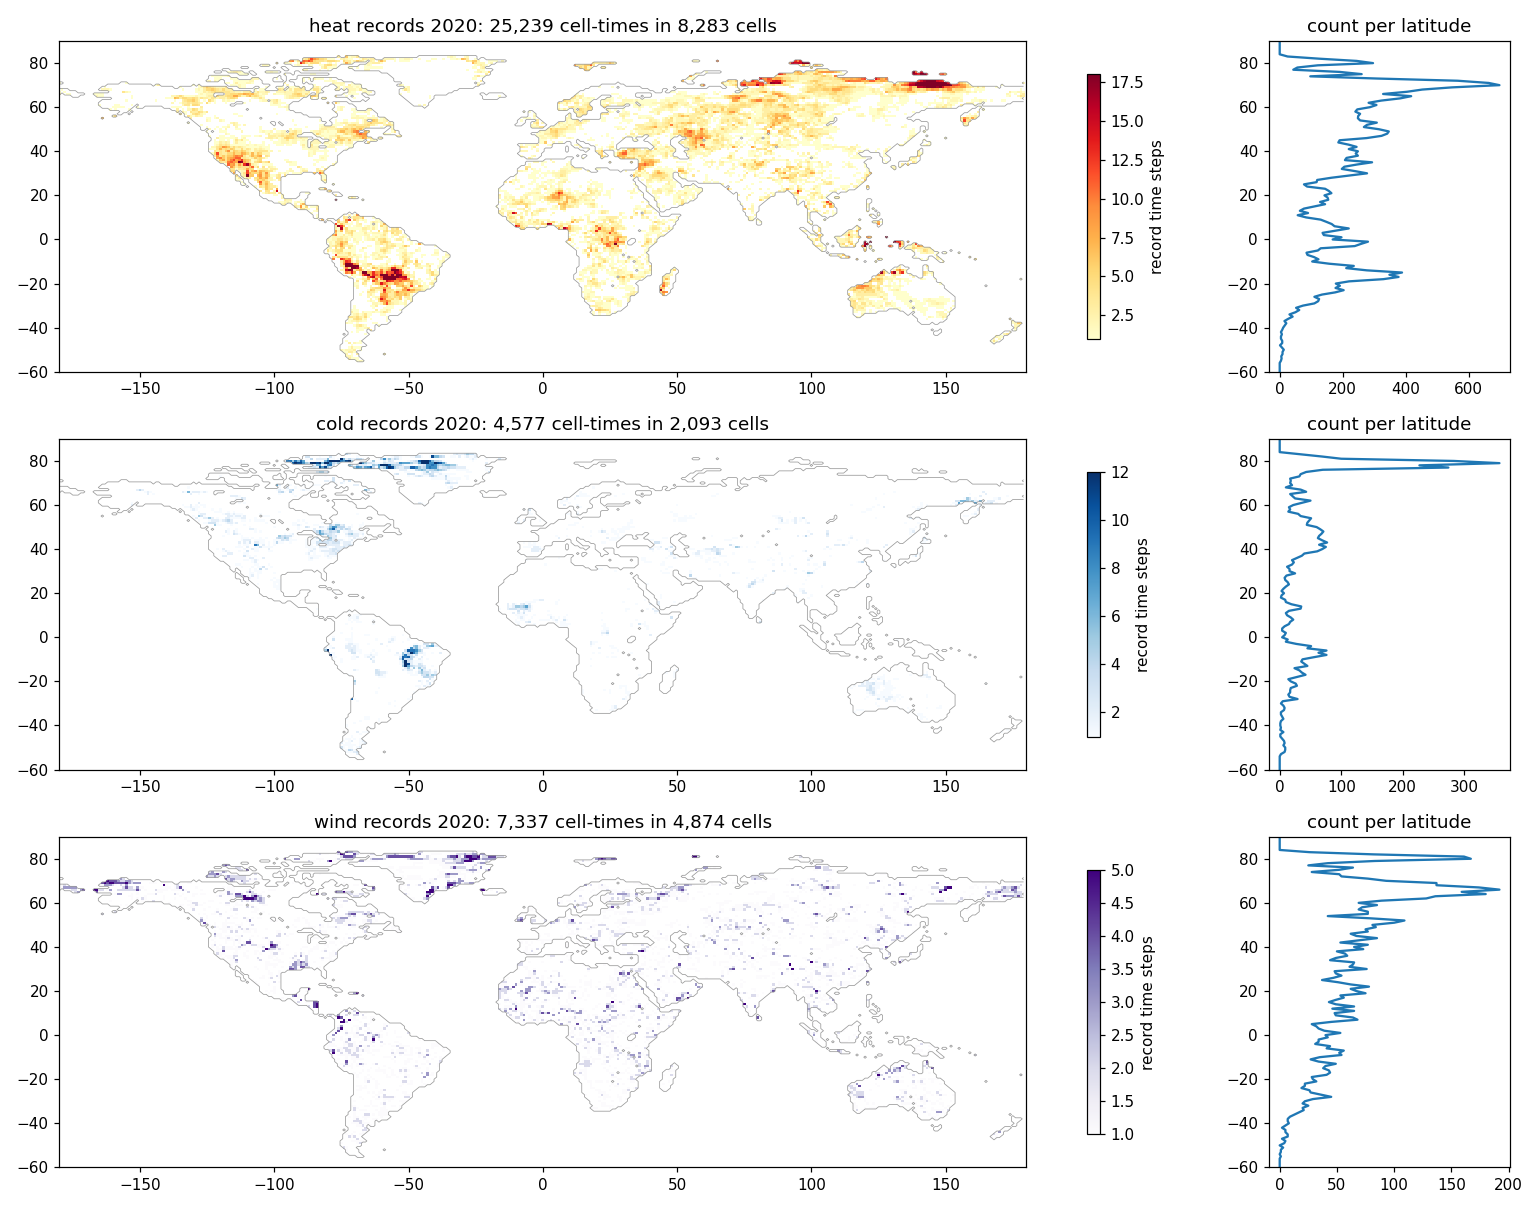
\includegraphics[width=0.72\linewidth]{records_2020_maps.png}
\caption{Record cell-times of 2020 against the 1979--2015 monthly extremes. Colour shows how many 6-hourly
time steps each cell broke its record; the right panels count records per latitude. Heat records dominate,
with the largest clusters in Arctic Siberia and central South America.}
\label{fig:records}
\end{figure}

\paragraph{Step 2: grouping records into events with DBSCAN.}
A heatwave is not one grid cell at one time but hundreds of neighbouring cells over several days. To forecast and score
\emph{events}, we need to group record cell-times that belong together, without knowing in advance how many events there
are or what shape they have. DBSCAN~\cite{ester1996dbscan} is designed for exactly this. It calls a point a \emph{core point} if
at least \texttt{min\_samples} points lie within a radius \texttt{eps}. Clusters grow by chaining core points that lie within reach of
one another, and points that are not reachable are labelled noise. Unlike K-means, it needs no number of clusters and finds
irregular shapes, like a heatwave that drifts east.

The key design choice is the distance. We embed each record cell-time in space and time: position on the sphere as 3D unit-sphere coordinates
(so that distance is the chord through the Earth and 1$^\circ$ of longitude near the pole is not treated as 111\,km) scaled so that
\textbf{250\,km} equals one unit, and time scaled so that \textbf{12\,h} equals one unit. Two records 250\,km apart at the same time, or at the
same place 12\,h apart, are therefore equally ``close''. With \texttt{eps}\,=\,1 and \texttt{min\_samples}\,=\,5 a point needs four other records
within that space--time neighbourhood to seed an event. Separate runs are made for heat, cold and wind. We chose \texttt{eps} with the
standard \emph{k-distance plot} (Figure~\ref{fig:kdist}): sort all points by the distance to their 5th neighbour and look for the knee
where the distance shoots up; points above the knee are isolated. For heat and cold the knee sits right at 1; wind records are
more scattered, consistent with gusty, short-lived wind extremes. The result is \textbf{1{,}220 events} (802 heat, 141 cold, 277 wind) that contain 78\%, 80\% and 57\%
of the heat, cold and wind records (Figure~\ref{fig:events}a); the rest are isolated cell-times treated as noise.


\paragraph{Step 3: which events are record-shattering? Isolation Forest.}
Zhang et al.\ found that the forecast error grows with the size of the exceedance, so we need to know which events are not just
records but \emph{exceptional} records. Every event is described by four features: number of cells (size), duration, peak exceedance and
area-weighted mean exceedance. An Isolation Forest~\cite{liu2008isolation} builds many random trees; each tree splits the data on a random feature at a random threshold until every point
is isolated. Anomalous points sit far from the bulk and are isolated after few splits, so the average path length
is a natural anomaly score that needs no distributional assumptions. Because the result depends on the random trees, we train
\textbf{20 forests with different seeds} (contamination 0.1) and call an event \emph{record-shattering} if it is flagged in at least
80\% of them \emph{and} its peak exceedance is above the median. The second condition removes events that are unusual only
because they are tiny or oddly shaped. This yields \textbf{91 record-shattering events}: 61 heat, 10 cold and 20 wind (Figure~\ref{fig:outliers}).

\begin{figure}[t]
\centering
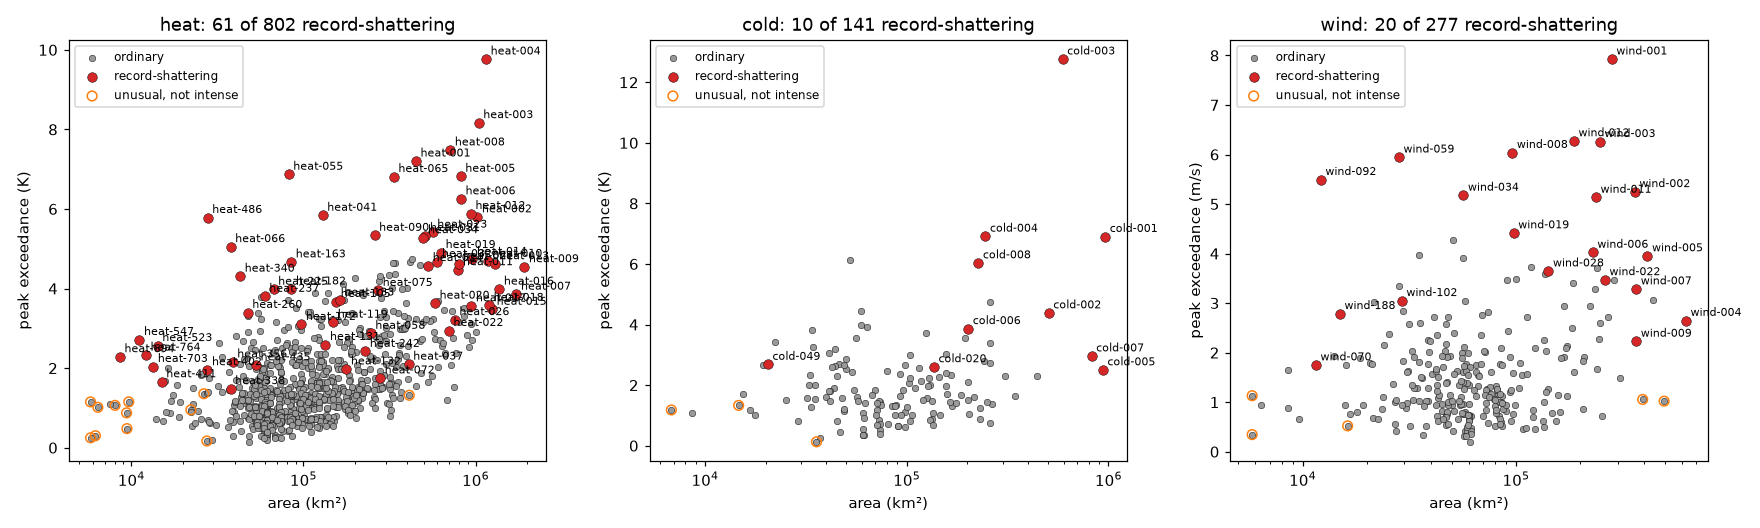
\includegraphics[width=0.9\linewidth]{events_2020_outliers.png}
\caption{Isolation Forest on event features: each dot is a DBSCAN event (area vs.\ peak exceedance). Red: record-shattering (flagged by $\geq$80\% of 20 forests and
above-median peak); orange circles: unusual in shape but not intense, therefore excluded. The Siberian heatwave (heat-004, almost 10\,K above the record)
and the North American cold outbreak (cold-003, 12.8\,K) stand out.}
\label{fig:outliers}
\end{figure}

\paragraph{Step 4: in which weather pattern did each event occur? K-means regimes.}
Forecasters describe the large-scale weather by its pattern at 500\,hPa (about 5.5\,km up): ridges (high pressure, sinking, clear skies, heat)
and troughs (low pressure, storms, cold air). A small set of recurring patterns, \emph{weather regimes}, captures much of
this variety~\cite{michelangeli1995regimes}. For each of six sectors (Middle East, North America, Euro-Atlantic, Asia--Siberia, South America, Australia)
we take daily 500\,hPa height anomalies from 1979--2020, with the seasonal cycle and the warming trend removed, and reduce them to 10
principal components. We then cluster the days with K-means~\cite{lloyd1982kmeans}. K-means places $k$ centres and alternates between
assigning each day to the nearest centre and moving each centre to the mean of its days, which minimises within-cluster variance.
Each centre is then a typical weather map. The silhouette score~\cite{rousseeuw1987silhouettes}, which compares how close a day is to its own cluster
versus the next one, chose $k=3$ in every sector. Values were low (0.10--0.18), as is typical: the atmosphere moves continuously
between patterns rather than in clearly separated states. The regimes are physically meaningful (Figure~\ref{fig:regimes}): for example, a Scandinavian blocking high
in the Euro-Atlantic sector and a Siberian ridge in Asia. Each event receives the regime of its sector on its days, which lets us check
that the case studies cover different circulation types.


\paragraph{Step 5: choosing the case studies.}
Events were ranked by area-weighted exceedance. We skipped events centred north of 75$^\circ$N, mostly over the coast, or with fewer than 5 cells, and
applied a quota so that the Middle East is represented. This gave \textbf{14 case studies} covering five sectors and all three regimes:
five heat events (including the Siberian heatwave, a Canadian Arctic event and the Levant heatwave of September 2020), four cold events (including the
October North American outbreak) and five wind events (including an Alaskan storm and Hurricane Laura's landfall). Eight of them are record-shattering. Each event is forecast
from 1, 3, 5 and 7 days before its peak, and scored on its 10{,}766 record cell-times.

\subsection{How forecasts are scored}
\label{sec:scores}
For each record cell-time we compare the forecast with ERA5. The \textbf{intensity error} is forecast minus truth (sign flipped for cold,
so that negative always means ``too mild''); the \textbf{hit rate} is the share of record cell-times at which the forecast also breaks the record.
Because record cells within one event are strongly correlated, uncertainty is estimated by a \textbf{bootstrap over events}~\cite{efron1994bootstrap}
(resampling whole events, not cells) and by leaving each event out in turn. Comparisons between two systems are \emph{paired}: they use the same
record cells. For probabilistic forecasts we use the Brier score~\cite{brier1950verification} and reliability diagrams.
For ordinary weather we use latitude-weighted RMSE, anomaly correlation (ACC) and \emph{activity}, the
spatial standard deviation of the forecast anomaly divided by that of ERA5, which measures \textbf{sharpness} (1 = as detailed as reality, $<1$ = smoothed).

\subsection{Remedy 1: PBC-inspired statistical correction}
\label{sec:pbc}
We learn three corrections per grid cell and lead time for 2\,m temperature and 10\,m wind speed, from 781 GraphCast hindcasts of 2016--2019
started within $\pm 7$ days of the same calendar date as each 2020 forecast (about 60 per start):
\begin{itemize}[leftmargin=*]
  \item \textbf{Debias}: subtract the mean hindcast error, $\hat y = f - \overline{(f - y)}$;
  \item \textbf{Persistence}: regression $\hat y = a + b f + c\, y_0$ on the forecast $f$ and the observed state $y_0$ at the start;
  \item \textbf{PBC}: the average of the two, as in Guan et al.
\end{itemize}
In a second, probabilistic check we attach a Gaussian spread learned from the hindcast errors, turning each forecast into
a probability of breaking the record. Note that this is a \emph{simplified adaptation}. Guan et al.\ correct ensemble forecasts at weeks 3--4 and
output quintile probabilities from about 20 years of reforecasts; we correct a single 1--10 day forecast from 4 years.
We therefore call it \emph{PBC-inspired}: it tests the idea of learning a model's errors from past forecasts, applied to short-range extremes.

\subsection{Remedy 2: conservation schemes inside GraphCast}
\label{sec:physics}
\paragraph{Intuition.}
The atmosphere neither creates nor destroys air, water or energy: the total amount of dry air is fixed; global water vapour changes only by
evaporation minus precipitation; total energy changes only by the radiation and heat that cross the top of the atmosphere and the surface.
An AI model learns none of these laws explicitly and can slowly drift. A conservation scheme measures the global budget after each 6\,h step and
applies the smallest uniform rescaling that restores it.

\paragraph{Implementation.}
\begin{enumerate}[leftmargin=*]
  \item \textbf{New outputs.} We added 7 output channels to GraphCast\_small for the fluxes (Section~\ref{sec:data}), initialised by copying existing
  output weights, so that before training the model is identical to \R{0}.
  \item \textbf{Schemes in the loop.} Following Sha et al., the schemes run inside the forecast loop, and the training loss is computed \emph{after} them,
  so the network learns to work with the constraints: non-negativity of humidity and precipitation; \emph{dry-air mass} (rescaling humidity at and below 600\,hPa);
  \emph{moisture} (rescaling precipitation so that the change in global water vapour equals evaporation minus precipitation);
  and \emph{total energy} (a factor $\gamma$ on temperature so that the change in total energy equals the net predicted fluxes).
  \item \textbf{Four runs}, identical in everything else: \R{1} control (new outputs, no schemes), \R{2} + mass, \R{3} + mass and moisture,
  \R{4} + mass, moisture and energy. Comparing \R{2}--\R{4} with \R{1}, rather than with \R{0}, isolates the effect of the physics from the effect of fine-tuning itself.
  \item \textbf{Adaptation.} GraphCast lives on fixed pressure levels and has no surface-pressure output. On fixed levels, conserving dry-air mass
  is equivalent to keeping global water vapour constant. With the moisture scheme on top, global precipitation then equals global evaporation every 6\,h.
\end{enumerate}

\paragraph{Training.}
Training used 2010--2014 and validation 2015, on one H100 per run. A first schedule with mostly single-step training improved one-step skill by 5\%
but made 5-day forecasts 15\% worse than \R{0}. A diagnostic run showed that the fluxes were not responsible: single-step training undoes GraphCast's original multi-step training,
which had taught it how to handle uncertainty over several days. The final schedule first trains only the new flux channels (1{,}500 steps, rest frozen; \R{1} stays identical to \R{0}),
then fine-tunes the whole model on 2-, 4- and 8-step rollouts (4{,}000 steps, learning rate $3\times10^{-6}$).

% =====================================================================
\section{Results}
\label{sec:results}

\subsection{Baseline: GraphCast\_small forecasts records as too mild}
\label{sec:res-base}
Table~\ref{tab:baseline} and Figure~\ref{fig:baseline} reproduce Zhang et al.'s finding on our events. Every kind of record is forecast as too
mild, and the shortfall grows from 1--2 units one day ahead to 5--7 units a week ahead. The hit rate falls accordingly: 65\% of heat records are
forecast one day ahead, but only 28\% a week ahead, and almost no wind records are forecast a week ahead. The error grows with the exceedance:
record-shattering heat events are underestimated by 3.3\,K on average, ordinary heat records by 1.1\,K. Events differ strongly. The Levant heatwave is
forecast almost perfectly even 7 days ahead (Figure~\ref{fig:eventmap}), while one South American cold event is never forecast as a record.
On ordinary days the same model is very skilful (2\,m temperature RMSE 0.68\,K at 1 day), so the weakness is specific to the extremes.

\begin{table}[t]
\caption{Baseline \R{0}: intensity error (negative = too mild) / hit rate on the record cell-times of the 14 events, by forecast start before the peak.}
\label{tab:baseline}
\centering\small
\begin{tabular}{lcccc}
\toprule
Start before the peak & $-1$\,d & $-3$\,d & $-5$\,d & $-7$\,d \\
\midrule
Heat (K)    & $-1.14$ / 65\% & $-2.10$ / 50\% & $-3.68$ / 33\% & $-5.18$ / 28\% \\
Cold (K)    & $-1.98$ / 42\% & $-2.24$ / 41\% & $-5.48$ / 22\% & $-5.58$ / 20\% \\
Wind (m/s)  & $-1.60$ / 42\% & $-2.33$ / 35\% & $-3.86$ / 19\% & $-7.49$ / \phantom{0}3\% \\
\bottomrule
\end{tabular}
\end{table}




\subsection{Do the schemes work, and do they do harm? Ordinary weather}
\label{sec:res-ordinary}
Before asking whether the physics helps records, we check that the schemes work and do not degrade everyday forecasts, as Sha et al.\ claim
(the statistical corrections are checked on ordinary weather in Section~\ref{sec:res-pbc}).

\paragraph{The budgets close.}
Each scheme closes its budget to rounding level in 4-step forecasts: the largest relative gap falls from $1.8\times10^{-5}$ to $2.2\times10^{-7}$ for mass, from
$6.8\times10^{-3}$ to $2.3\times10^{-7}$ for moisture and from $8.2\times10^{-5}$ to $2.4\times10^{-7}$ for energy. On the 2015 validation (Table~\ref{tab:val}) mass and moisture
cost nothing relative to the control \R{1}, while energy costs about 5 points more at 5 days. The energy cost appears before any training of the backbone, so it comes from the predicted
fluxes: small systematic errors in their global totals shift the global temperature every step, and the shifts accumulate.


\paragraph{52 ordinary dates.}
We then checked everyday skill with 10-day forecasts from 52 weekly dates of 2020, scored globally with 95\%
bootstrap intervals over the dates (Figure~\ref{fig:ordinary}, Table~\ref{tab:ordinary}).
\begin{itemize}[leftmargin=*]
  \item \textbf{Fine-tuning trades lead times.} \R{1} beats \R{0} at 1 day on every variable (wind and 850\,hPa temperature on 100\% of dates), is 1--2.5\% worse at
  3--5 days for temperature and wind, and returns to \R{0}'s level by 7--10 days.
  \item \textbf{Mass and moisture are free.} \R{2} and \R{3} stay within about 1 percentage point of \R{1} at every lead time; anomaly correlation agrees to 0.01.
  They also fix a real drift: \R{0} slowly moistens the atmosphere, reaching +1.55\% global water vapour after 10 days. \R{2}--\R{4} hold it at +0.15\%,
  which is ERA5's own natural variation.
  \item \textbf{Energy is not free.} \R{4} is the worst model at 3--7 days on every variable; its 2\,m temperature error is +6.8\% at 5 days and +11.3\% at 10 days
  and worse than \R{0} on every one of the 52 dates at 3 and 5 days. Its total energy ends furthest of all models from ERA5's
  ($+1.6\times10^{-3}$ relative), the opposite of the scheme's intent. Its temperature fields become \emph{noisier} than reality (activity 1.08 at 10 days) while its pressure fields
  become the smoothest.
\end{itemize}


\begin{figure}[t]
\centering
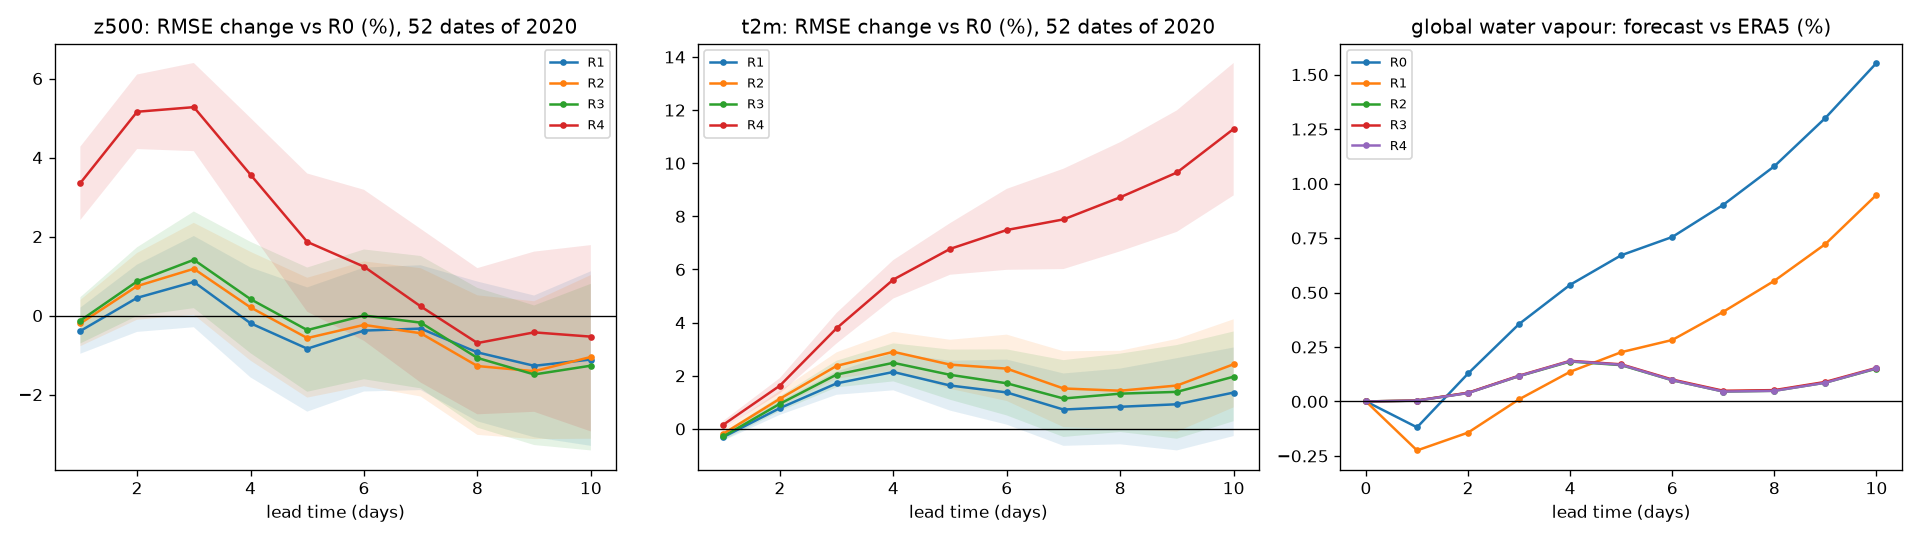
\includegraphics[width=0.88\linewidth]{ordinary_skill.png}
\caption{Ordinary weather on 52 dates of 2020. Left and centre: RMSE change against \R{0} for 500\,hPa height and 2\,m temperature, with 95\% bootstrap ranges.
Right: global water vapour of each forecast relative to ERA5. GraphCast\_small (\R{0}) drifts moist; the mass scheme (\R{2}--\R{4}) removes the drift.}
\label{fig:ordinary}
\end{figure}
So mass and moisture conservation fix a genuine drift for free; whether that helps \emph{records} is the question of Section~\ref{sec:res-physics}.


\subsection{Remedy 1: statistical correction makes records worse}
\label{sec:res-pbc}
On ordinary weather in the event boxes, the corrections work as intended: with PBC, RMSE falls from 2.62 to 2.57\,K for temperature and from
1.78 to 1.62\,m/s for wind. On the records, however, they do not help (Table~\ref{tab:pbc}, Figure~\ref{fig:pbc}). Debias changes little.
Persistence and PBC make heat records much worse: at $-7$\,d the heat error goes from $-5.18$\,K to $-7.49$\,K with PBC, and the hit rate falls from 28\% to 5\%.
The worsening at $-5$\,d holds in 5 of 5 heat events under bootstrapping and leave-one-out; Debias is the only correction with a small consistent gain, for wind (+0.2--0.3\,m/s).

The correction is learned from mostly ordinary days by minimising average error, so for an uncertain forecast it moves toward the usual conditions, exactly the wrong direction when something unprecedented happens.

\begin{table}[t]
\caption{Intensity error on record cell-times with the statistical corrections, starts $-5$\,d / $-7$\,d (negative = too mild).}
\label{tab:pbc}
\centering\small
\begin{tabular}{lcccc}
\toprule
 & \R{0} & Debias & Persistence & PBC \\
\midrule
Heat (K)   & $-3.68$ / $-5.18$ & $-3.98$ / $-5.34$ & $-5.80$ / $-9.64$ & $-4.89$ / $-7.49$ \\
Cold (K)   & $-5.48$ / $-5.58$ & $-5.20$ / $-5.35$ & $-5.58$ / $-7.17$ & $-5.39$ / $-6.26$ \\
Wind (m/s) & $-3.86$ / $-7.49$ & $-3.53$ / $-7.21$ & $-5.62$ / $-8.57$ & $-4.58$ / $-7.89$ \\
\bottomrule
\end{tabular}
\end{table}


\paragraph{The probabilistic view helps.}
Turning forecasts into probabilities of breaking the record changes the picture (Figure~\ref{fig:prob}). Every version beats \R{0}'s yes/no forecast
on the Brier score (skill 0.05--0.34), but most of the gain comes from adding uncertainty alone: ``\R{0} + spread'' is the best heat forecast.
Probabilities are reliable for heat, overconfident for cold and too cautious for wind with Persistence and PBC. At a 20\% warning level, the share of
heat records caught 5 days ahead rises from 30\% to 65\%, while the share of correct warnings falls from 66\% to 41\%, a classical trade-off between
missed events and false alarms~\cite{gneiting2007probabilistic}.



\subsection{Remedy 2: conservation schemes on the records}
\label{sec:res-physics}
\paragraph{But they do not help records.}
On the 14 events (Figure~\ref{fig:physics}), \R{2} and \R{3} are indistinguishable from the control \R{1}: changes are mostly within $\pm0.15$\,K or m/s.
\R{4} is consistently worse from $-1$ to $-5$\,d: for example, cold at $-3$\,d by $-0.45$\,K (in 4 of 4 events), wind at $-3$\,d by $-0.46$\,m/s (5 of 5) and heat at $-5$\,d
by $-0.90$\,K, with hit rates falling by up to 10--14 points. The fine-tuning shared by all physics runs (\R{1} vs.\ \R{0}) does improve heat at long leads: at $-7$\,d the heat error goes from
$-5.18$ to $-4.11$\,K and the hit rate from 28\% to 37\%; record-shattering heat improves from $-3.34$ to $-2.98$\,K on average. Cold and wind are mixed.

\begin{figure}[t]
\centering
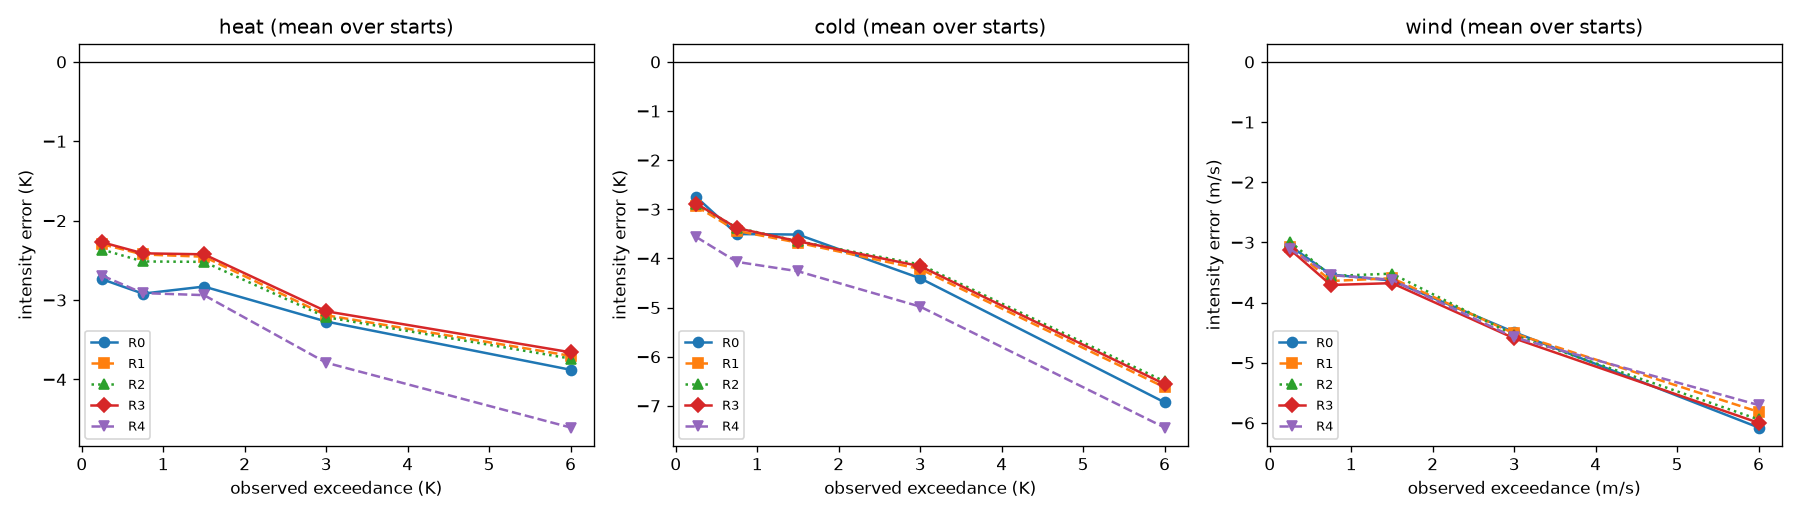
\includegraphics[width=0.85\linewidth]{comparison_physics_bias_vs_exceedance.png}
\caption{Intensity error against exceedance for \R{0} and the fine-tuned runs. \R{1}--\R{3} lie on top of each other (the physics changes nothing) and above \R{0} for heat
(the fine-tuning helps); \R{4} (energy) is the worst for heat and cold.}
\label{fig:physics}
\end{figure}

\paragraph{Why does fine-tuning help heat? Sharpness.}
Figure~\ref{fig:sharp} measures how detailed the forecasts are in the event boxes. \R{0} becomes steadily smoother up to day 7 (2\,m temperature
activity 0.944), while the fine-tuned runs stay near 0.97. A smoother forecast cannot reach a record value, so the fine-tuned runs, which blur less,
get closer to the records. This is consistent with the hedging explanation in Section~\ref{sec:overview}.



% =====================================================================
\section{Discussion and conclusions}
\label{sec:conclusions}

\paragraph{Record extremes are a problem of the tails and of smoothing, not of global balance.}
\emph{Statistical correction fails} because it is trained on ordinary days to minimise average error: for an uncertain forecast the optimal move is toward the normal,
the wrong direction for a record. Its value lies in uncertainty, since as probabilities even uncorrected forecasts give useful record warnings.
\emph{Global constraints do not help} because a record is a regional anomaly: balancing global dry-air mass, water or energy changes global totals by tiny amounts
(ERA5 itself is out of balance by 0.0004--0.2\% on these levels) and says nothing about \emph{where} heat or wind concentrates. Mass and moisture conservation are
cheap and even fix a moistening drift, but act on the wrong scale. \emph{Energy conservation hurts} because it forces the budget to agree with the model's own predicted
fluxes, so any flux bias is pushed into the temperature every 6\,h; Sha et al.\ trained FuXi with the fluxes from the start, whereas we added them to a finished model.
\emph{What did help} is less smoothing: fine-tuning on short rollouts costs a little squared error at 3--5 days (+1--2.5\% on ordinary dates) but brings heat forecasts
about 1\,K closer to the records a week ahead. Squared-error training rewards exactly the smoothing that hides extremes.

\paragraph{Conclusion.} For record-breaking extremes, neither the PBC-inspired correction nor Sha et al.'s conservation schemes reduce GraphCast\_small's
underestimation. Mass and moisture conservation can be added at no cost in skill where physical consistency matters; energy conservation needs reliable fluxes first.
The more promising directions keep forecasts sharp and their tails wide.

\paragraph{Limitations.}
The conclusions rest on 14 events from one year and on one small model at 1$^\circ$; differences below about 0.2\,K should not be over-interpreted.
ERA5 is itself a smoothed reanalysis, and station records can be more extreme. The PBC-inspired correction is a deterministic, short-range adaptation and
does not test Guan et al.'s published subseasonal method. The schemes were adapted to pressure levels (so mass conservation amounts to fixed global water vapour),
and added by fine-tuning (5{,}500 steps on years the model already knew) rather than training from scratch.

% =====================================================================
\section{Prospects}
\label{sec:prospects}
The evidence points to three levers (sharp forecasts, weighted tails, probabilities); ideas in order of how directly our results support them:
\begin{enumerate}[leftmargin=*]
  \item \textbf{Tail-targeted post-processing}: quantile or extreme-value corrections fitted only to the most extreme days, per K-means regime.
  \item \textbf{More events and years}: all 91 record-shattering events of 2020 and the records of 2021--2023.
  \item \textbf{Sharpness-preserving training}: spectral, ``adjusted MSE'' or CRPS losses, since our only gain came from less smoothing.
  \item \textbf{Probabilistic forecasts}: ensembles or GenCast-like models~\cite{price2025gencast}; spread alone gave heat Brier skill 0.14--0.25.
  \item \textbf{Better inputs and physics}: soil moisture, oversampled extremes, jointly trained fluxes, 0.25$^\circ$ grid.
\end{enumerate}

\begin{ack}
Computations were run on the MBZUAI shared H100 cluster (one 6\,h forecast step takes 0.06\,s on an H100), Google Colab and a laptop. All code, scripts per phase, SLURM jobs and offline tests are in the project repository \texttt{graphcast-extremes}; its README lists the exact commands. We thank the authors of GraphCast, WeatherBench~2 and ARCO-ERA5 for making
their models and data openly available.
\end{ack}

\bibliographystyle{plainnat}
\bibliography{refs}

\appendix
\section{Additional figures and tables}
\label{app:figs}
These figures and tables support the main text; they are referenced where they are discussed.

\begin{figure}[h]
\centering
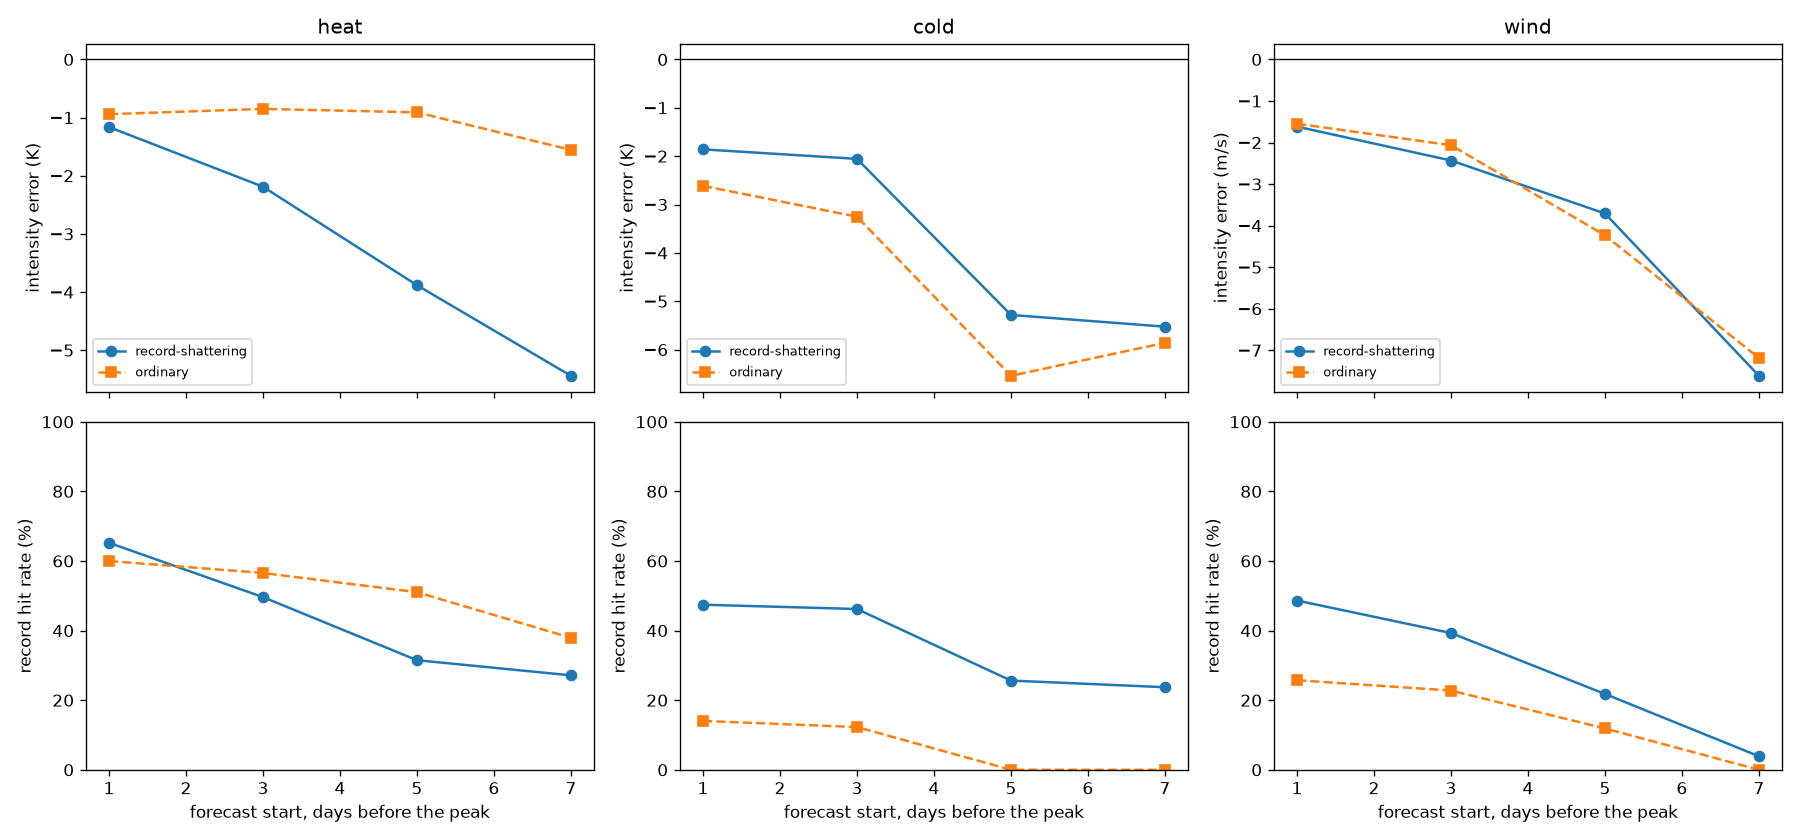
\includegraphics[width=0.92\linewidth]{R0_by_start.png}
\caption{Baseline \R{0} by forecast start: intensity error (top) and record hit rate (bottom), separately for record-shattering (blue) and ordinary
record events (orange). For heat, the record-shattering events degrade much faster with lead time.}
\label{fig:baseline}
\end{figure}

\begin{table}[h]
\caption{Ordinary weather, 52 dates of 2020: RMSE change against \R{0} (negative = better), and global water vapour of the forecast vs.\ ERA5 at 10 days.}
\label{tab:ordinary}
\centering\small
\resizebox{\linewidth}{!}{%
\begin{tabular}{lcccc}
\toprule
RMSE change vs.\ \R{0} & 1 day & 3 days & 5 days & 10 days \\
\midrule
2\,m temp.: \R{1} / \R{2} / \R{3} / \R{4} & $-0.3/-0.2/-0.3/+0.2$\% & $+1.7/+2.4/+2.0/+3.8$\% & $+1.6/+2.4/+2.0/+6.8$\% & $+1.4/+2.4/+2.0/+11.3$\% \\
z500: \R{1} / \R{4} & $-0.4/+3.4$\% & $+0.9/+5.3$\% & $-0.8/+1.9$\% & $-1.1/-0.5$\% \\
10\,m u-wind: \R{1} / \R{4} & $-1.9/-1.4$\% & $+1.1/+3.2$\% & $+1.5/+3.3$\% & $+0.8/+0.7$\% \\
\midrule
Water vapour at 10 d & \R{0} +1.55\% & \R{1} +0.95\% & \R{2}--\R{3} +0.15\% & \R{4} +0.15\% \\
\bottomrule
\end{tabular}}
\end{table}

\begin{table}[h]
\caption{Validation on 2015 (normalised loss on the core variables; lower = better).}
\label{tab:val}
\centering\small
\begin{tabular}{lccc}
\toprule
 & 6\,h & 1 day & 5 days \\
\midrule
\R{0} GraphCast\_small & 0.754 & 1.263 & 3.70 \\
\R{1} control (fine-tuned) & 0.738 & 1.240 & 3.86 (+4.3\%) \\
\R{2} + dry-air mass & 0.738 & 1.240 & 3.86 (+4.3\%) \\
\R{3} + moisture & 0.739 & 1.241 & 3.87 (+4.4\%) \\
\R{4} + energy & 0.754 & 1.258 & 4.04 (+8.9\%) \\
\bottomrule
\end{tabular}
\end{table}

\begin{figure}[h]
\centering
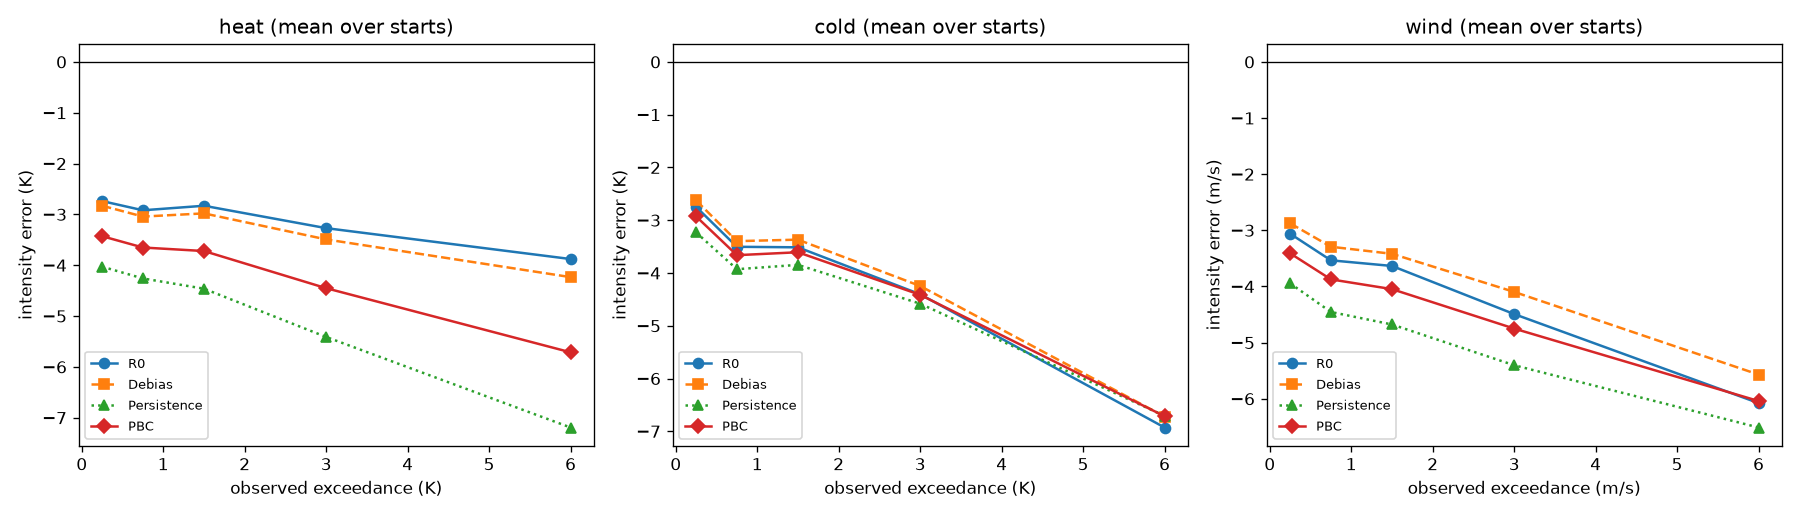
\includegraphics[width=0.95\linewidth]{comparison_bias_vs_exceedance.png}
\caption{Intensity error against observed exceedance, averaged over starts, for \R{0} and the three corrections. All curves slope downward: the
bigger the record, the larger the shortfall. Persistence and PBC shift heat further from zero.}
\label{fig:pbc}
\end{figure}

\begin{figure}[h]
\centering
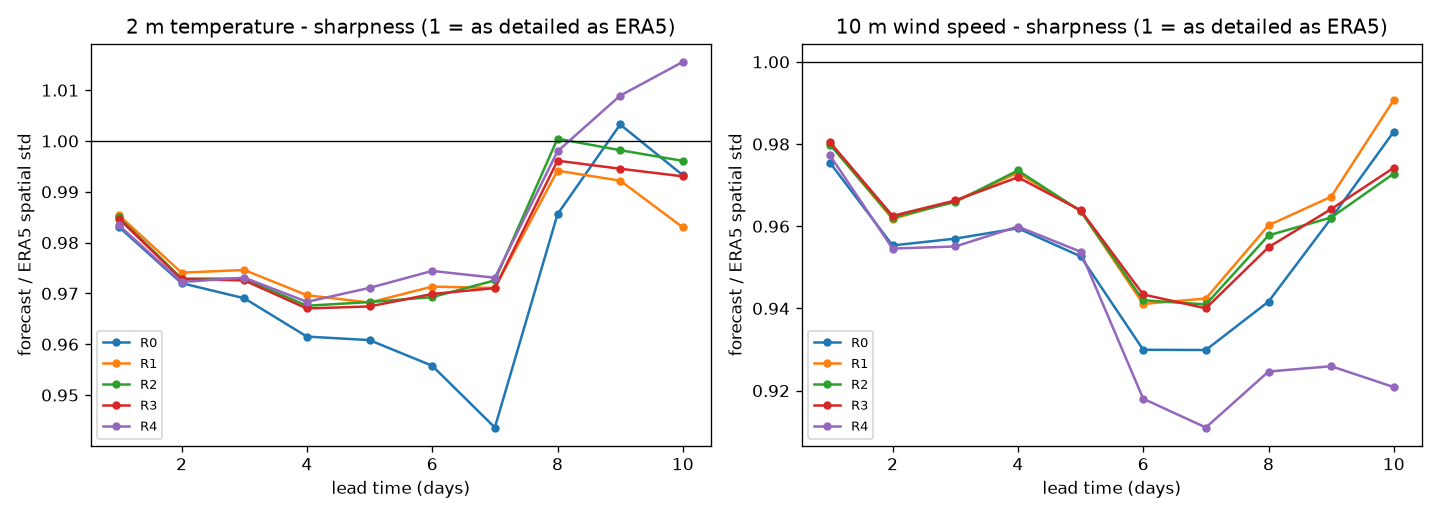
\includegraphics[width=0.85\linewidth]{sharpness.png}
\caption{Sharpness in the event boxes: spatial standard deviation of the forecast divided by that of ERA5 (1 = as detailed as reality). \R{0} smooths its
temperature forecasts up to day 7; the fine-tuned runs keep more detail. \R{4} has the smoothest wind.}
\label{fig:sharp}
\end{figure}

\begin{figure}[h]
\centering
\begin{subfigure}[b]{0.36\linewidth}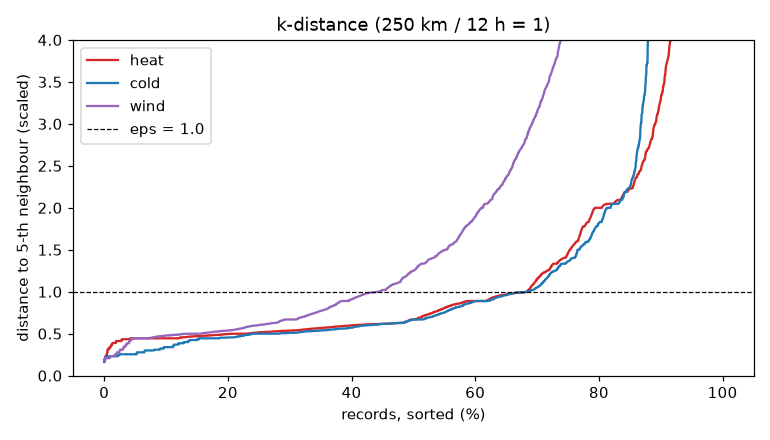
\includegraphics[width=\linewidth]{kdistance.png}\caption{}\label{fig:kdist}\end{subfigure}\hfill
\begin{subfigure}[b]{0.62\linewidth}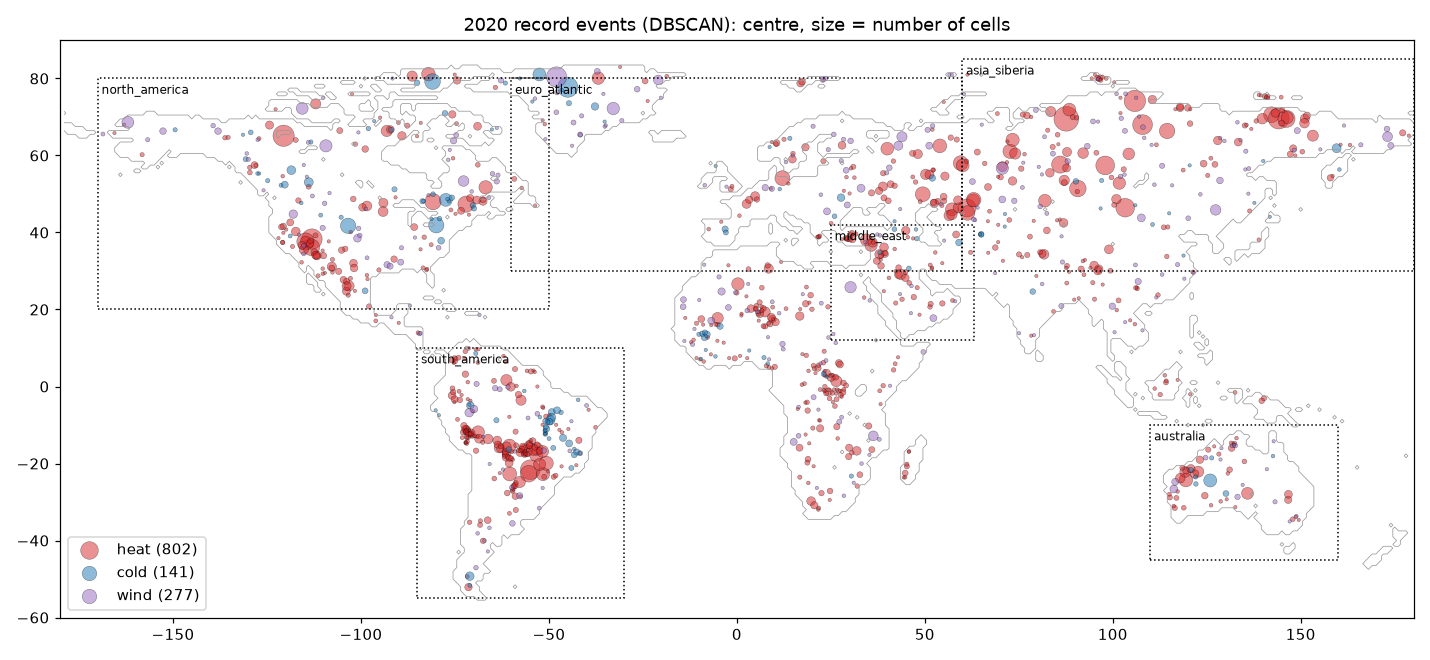
\includegraphics[width=\linewidth]{events_2020_map.png}\caption{}\end{subfigure}
\caption{(a) k-distance plot used to choose DBSCAN's \texttt{eps}: distance (in the 250\,km\,/\,12\,h unit) from each record cell-time to its 5th neighbour, sorted.
The knee near 1 separates dense events from scattered records. (b) Centres of the 1{,}220 DBSCAN events of 2020 (circle size = number of cells),
with the six regional sectors used for weather regimes.}
\label{fig:events}
\end{figure}

\begin{figure}[h]
\centering
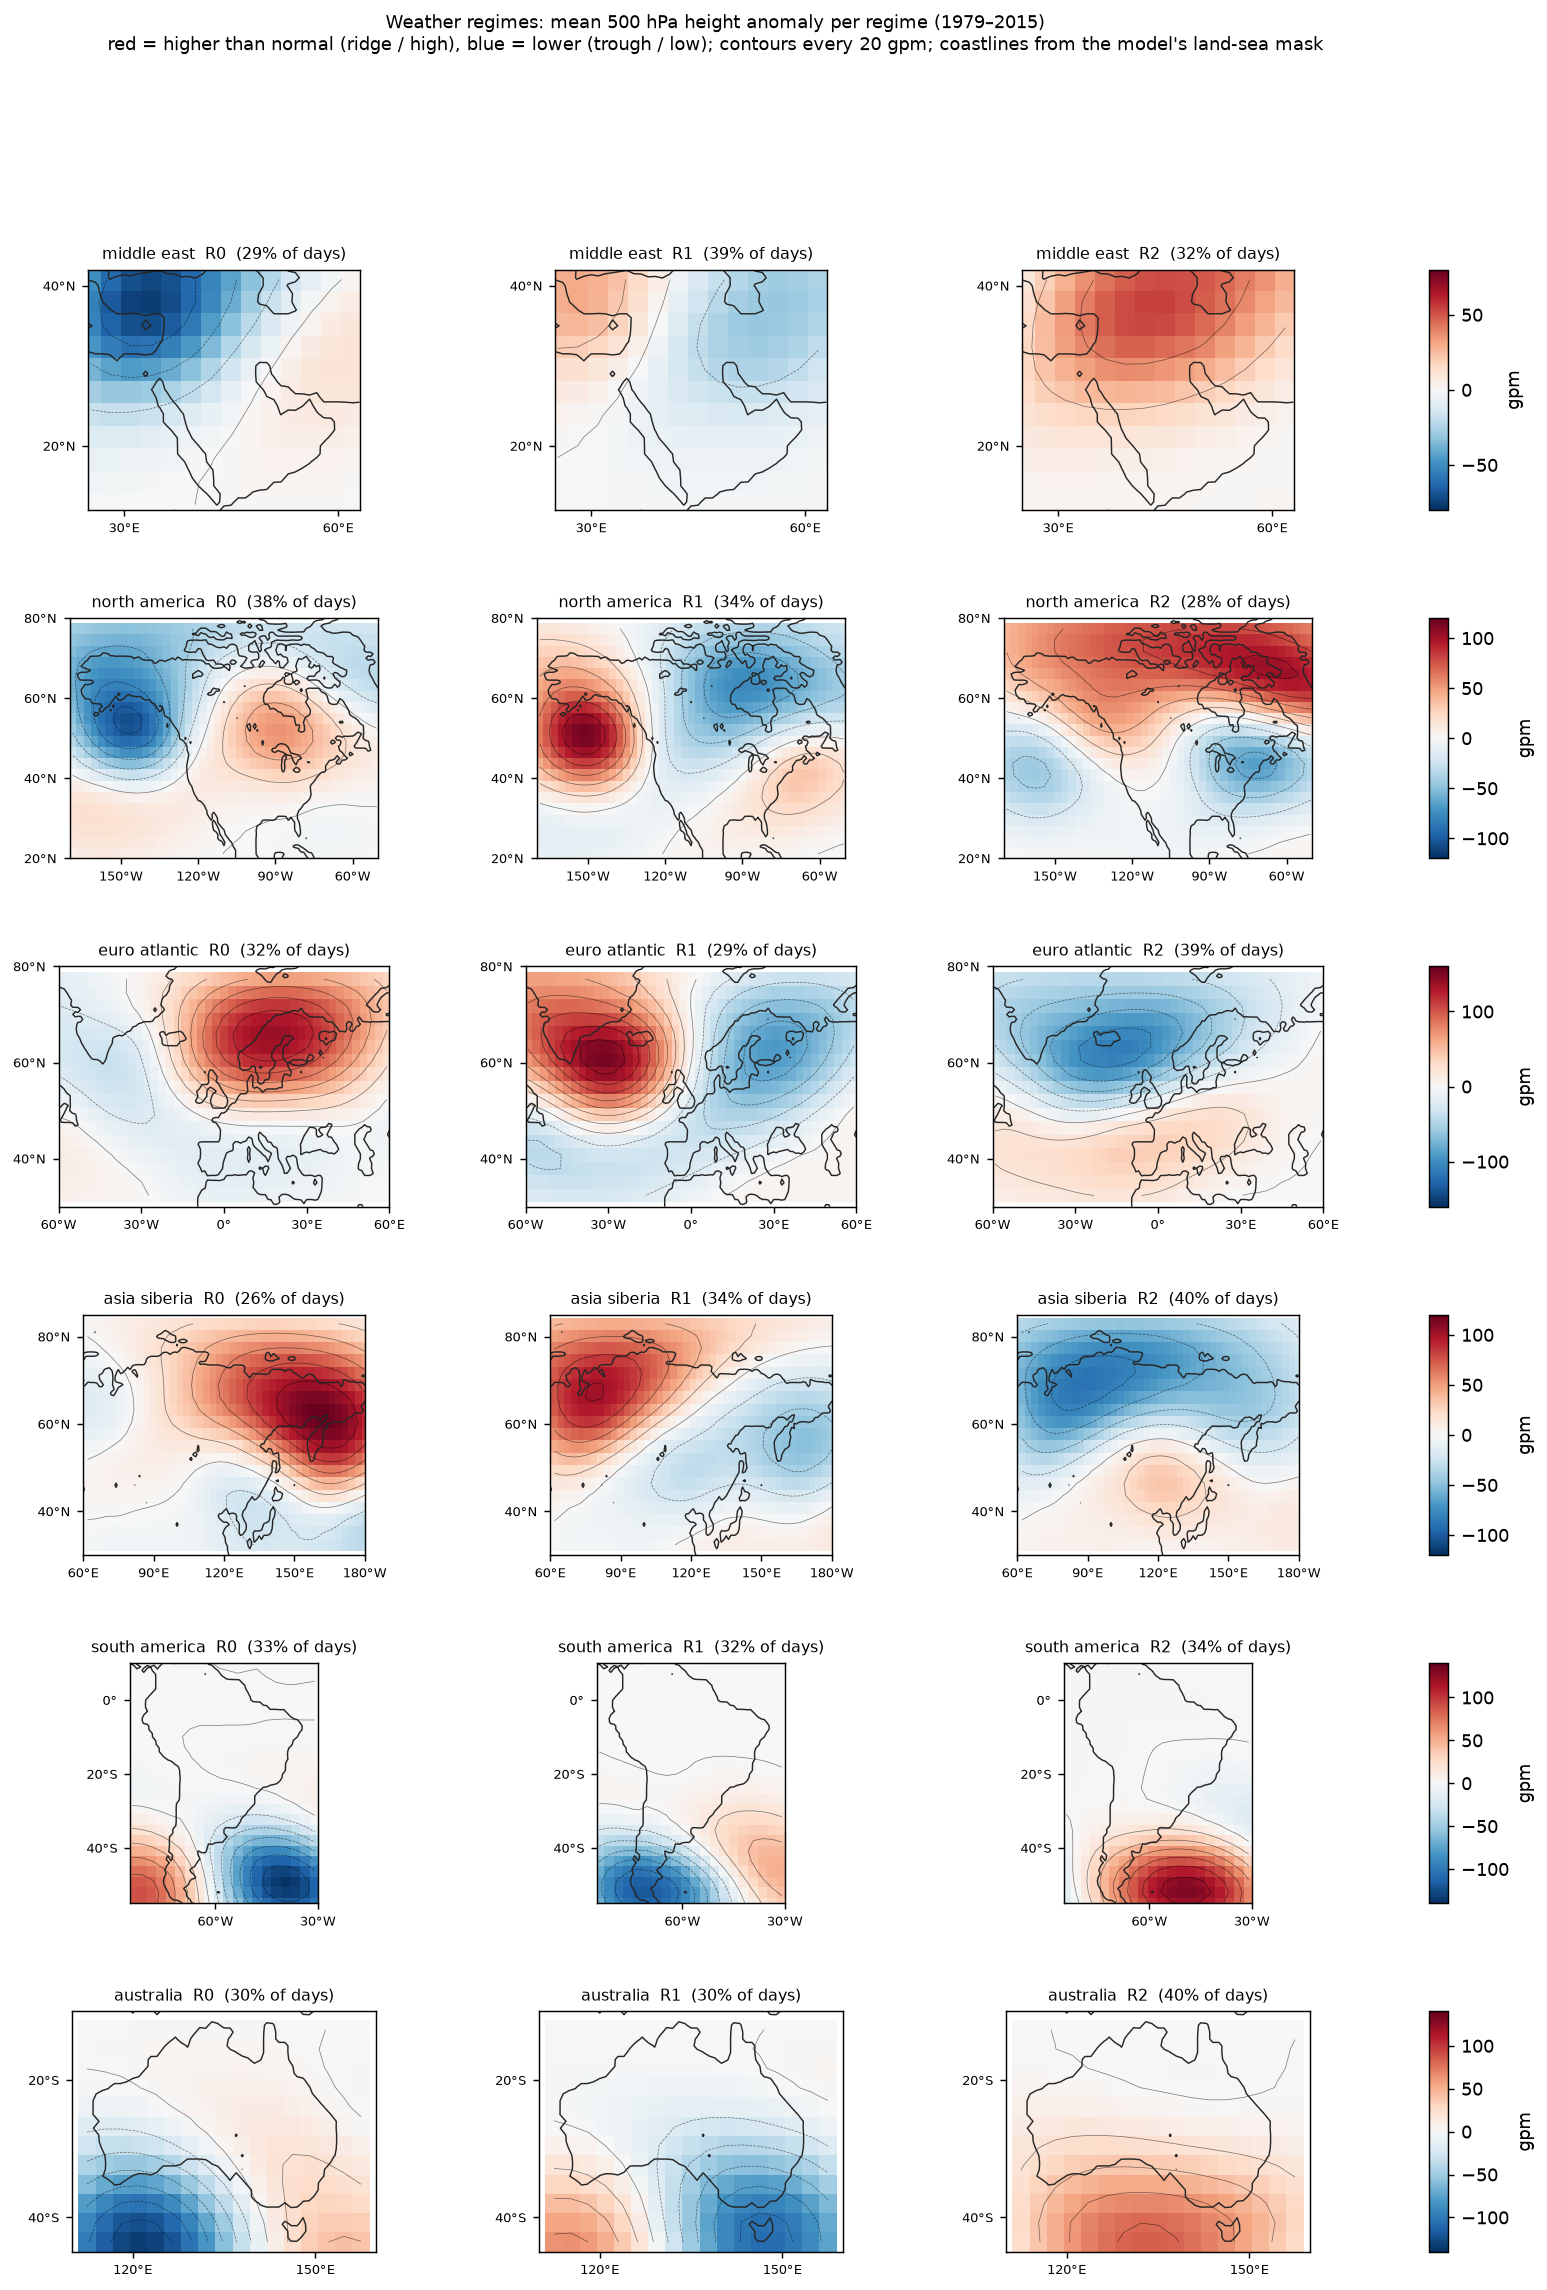
\includegraphics[width=0.66\linewidth,trim=0 0 0 120,clip]{regimes_composites.png}
\caption{K-means weather regimes ($k=3$ per sector): mean 500\,hPa height anomaly of each cluster, 1979--2015 (red = ridge/high, blue = trough/low),
with the share of days in each regime. Heat records tend to occur under ridges, cold records under troughs that let polar air move south.}
\label{fig:regimes}
\end{figure}

\begin{figure}[h]
\centering
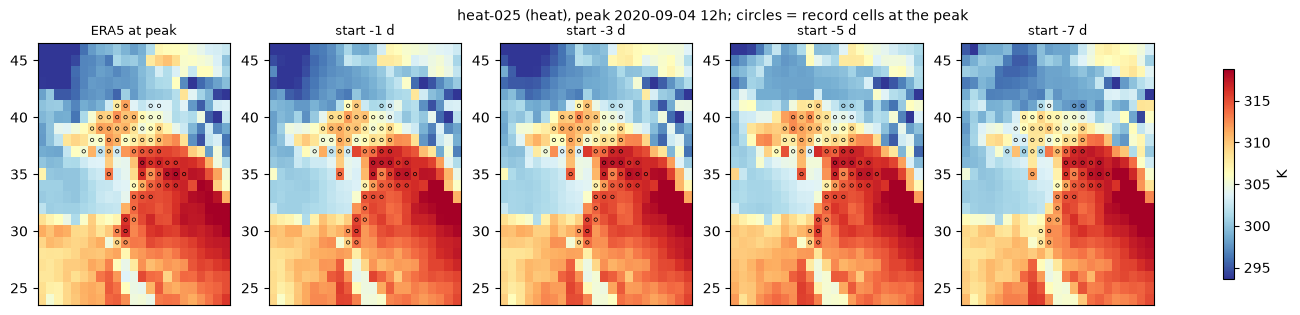
\includegraphics[width=\linewidth]{heat-025.png}
\caption{Example case study: the Levant heatwave of 4~September 2020 (heat-025). Left: ERA5 at the peak; then GraphCast\_small forecasts started 1, 3, 5 and 7 days earlier.
Circles mark record cells. This event is well forecast at all leads; most others are not.}
\label{fig:eventmap}
\end{figure}

\begin{figure}[h]
\centering
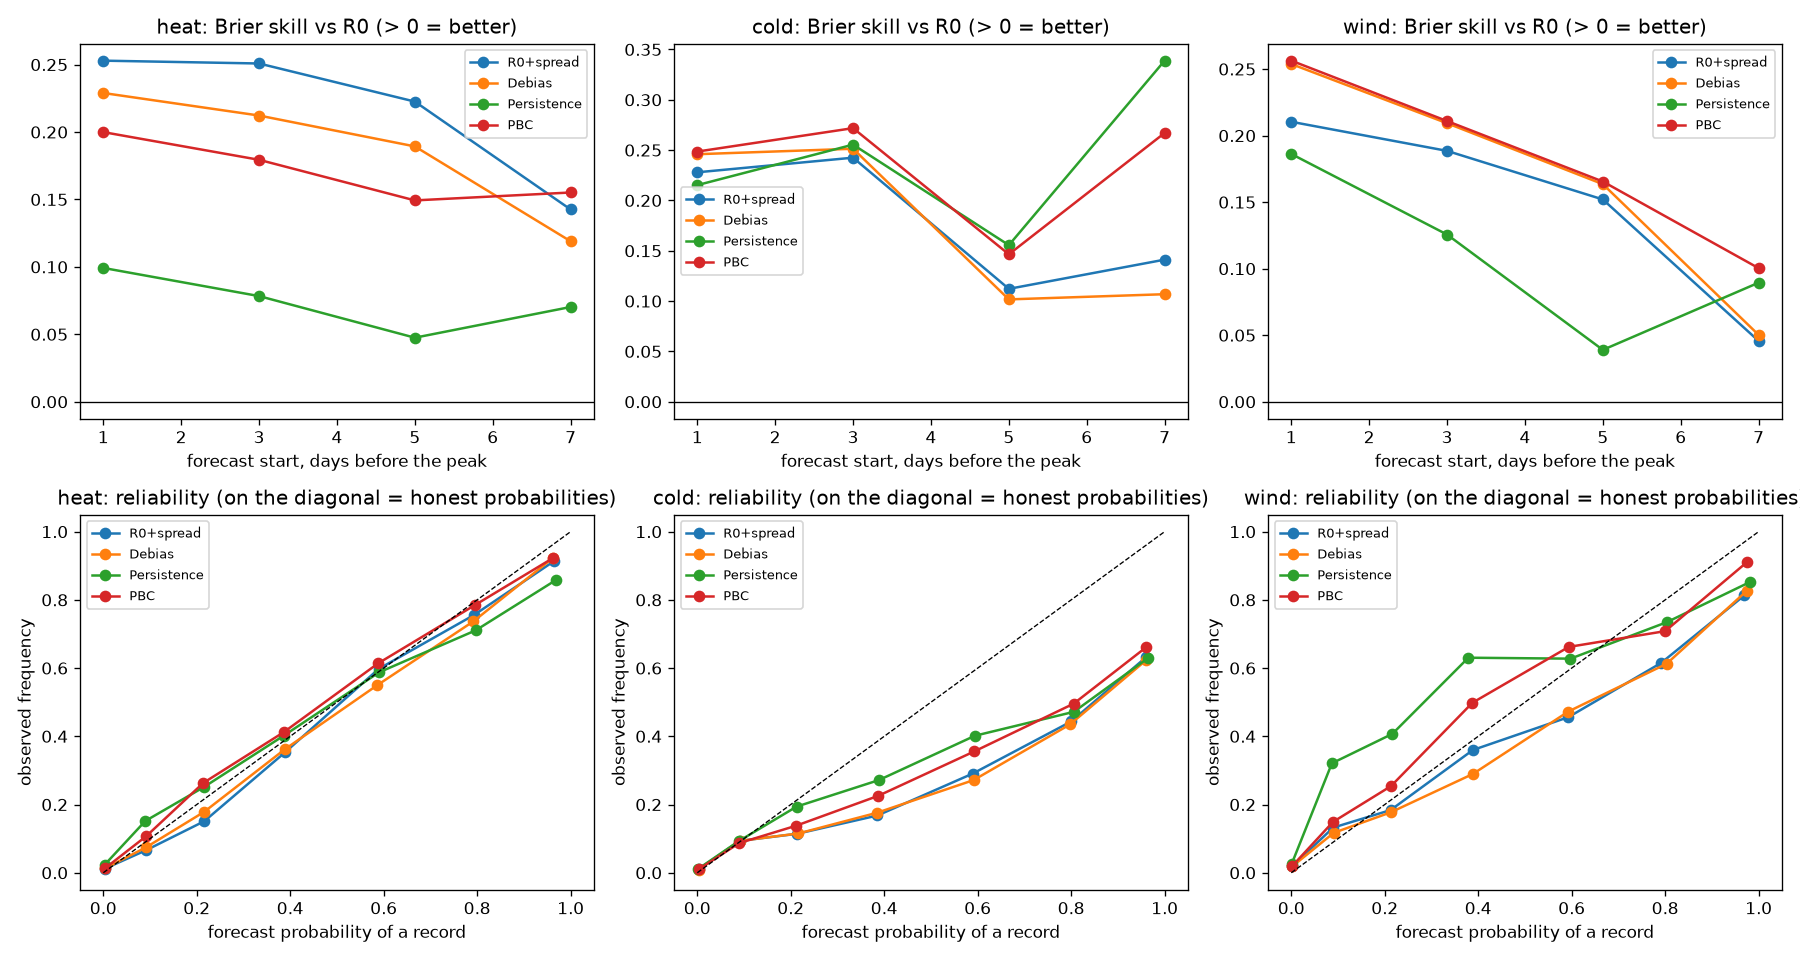
\includegraphics[width=0.95\linewidth]{record_probability.png}
\caption{Probabilistic check. Top: Brier skill relative to \R{0}'s yes/no forecast ($>0$ = better). Bottom: reliability diagrams; points on the diagonal mean the
forecast probabilities are honest. Adding a learned spread helps everywhere; the correction itself adds little beyond that.}
\label{fig:prob}
\end{figure}

\end{document}
